% !TEX encoding = UTF-8 Unicode
\chapter{Digitale Bildung}

\section{Einleitung und Motivation}

Da die digitalisierung einen immer größeren Teil in unserer Gesellschaft wird, wird es auch umso wichtiger die neue Generation darauf vorzubereiten. Es ist davon auszugehen, das sich durch die voraschreitende Automatisierung immer mehr Berufe von Maschinen und Computern ersetzt werden. Dadurch werde vermutlich einige Arbeitsplätze verloren gehen, aber gleichzeitig ergibt sich dadurch auch eine neue Chance: Die Logic für diese Automatisierung muss ja von jemanden entwickelt werde. Es wäre also nur zukunftsweisend  schon in der Schule den jungen Menschen unseres Landes die Kentnisse and die Hand zu geben, die ihnen in dem immer witchtiger werdenden Feld der Informatik weiterhelfen.
Die Informatik als Berufsfeld ist aber nicht der einzige Anwenungsfall in dem ein solcher UNterricht helfen kann. Das logische denken braucht jeder Mensch in seinem leben ganz egal ob er ein Computerprogramm schreiben will oder nur überlegt in weclher Reihenfolge er seine Kleidung anlegt. Heutzutage besitzt fast jeder junge Mensch ein Smartphone mit einer Internetverbindung das er den ganzen Tag  mit sich herumträgt. Wie diese aber funktioniert wissen ur die wenigsten so genau. 
Lernen die Schüler denn schon logisch zu denken, im Team zu arbeiten und können mit den dafür nötigen Werkzeugen umgehen? Mt diesen Fragen soll sich dieses Kapitel befassen und alternativ Lösungen anbieten wenn unser Bildungssystem diese nicht bietet.


\section{Stand der Dinge}

Um ein Bild über den Stand der Dinge des Informatik-Unterrichts zu bekommen wurde hier der Bildungsplan für Baden-Württemberg untersucht. Genauer gesagt der ab 2016 gültige Bildungsplan für die Grundschule und gemeinsamen Teil der Sekundarstufe I. Mit diesen beiden Schulstufen ist der Schulweg eines jeden Schülers in Baden-Würrtemberg abgedeckt und eignet sich somit sich ein Bild über den Bildungsstand der Allgemeinhiet Im Bereich Informtaik zu machen. Denn damit sind alle Schüler von der ersten bis zu 10. Klasse abgedeckt und ist somit die Bildung die theoretisch jeder Schüler in Baden-Würtemberg bekommt. Hier wird untersucht, welche gebiete der Informatik an den öffentlichen Schulen unterrichtet wird, und wie diese unterrichted werden, um eine Aussage darüber zu treffen, ob die aus der Einleitung gennanten Punkte bereits umgesetzt wurden.

\subsection{Grundschule}
Im Bildungsplan der Grundschule gibt es keinen eigenen Abschnitt für das Fach Informatik\cite{Fachuebersicht}.Und auch in ferner verwandten Fächer wie der Mathematik\cite{Mathematik} oder gar Sachunterricht\cite{Sachunterricht}  finden sich keine Teilgebiete die unbedingt mit der Informatik zu tun haben. Daraus kann der Schluss gezogen werden, dass die Infromatik als Fach in der Grundschule vom aktuellen Bildungsplan von Baden-Würtemberg so nicht vorgesehn ist.

\subsection{Sekundarstufe I}
Ab der Sekundarstufe I (also 5. - 10. Klasse) ist im gemeinsamen Bildungsplan für alle Schulsystem ein eigenes Fach für die Informatik vorgesehn, dass in mehrere Kompetenzen aufgegliedert wurde\cite{Informatik}. Folgende Infografik wurde zu diesen Verschiedenen Kompetenzen veröffentlicht:

\begin{figure}[ht]
	\centering
	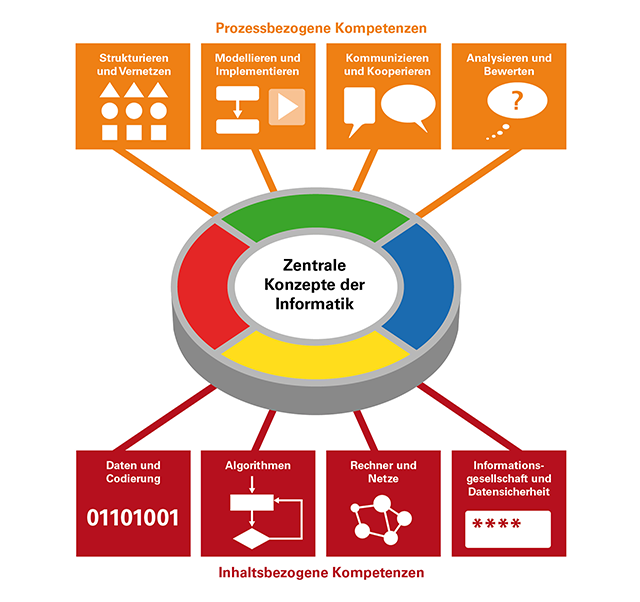
\includegraphics[width=\textwidth,height=\textheight,keepaspectratio]{images/BildungsplanInformatik.png}
	\caption{Infografik zu den Inhalten des Bildungsplans 2016 von Baden-Würtemberg für das Fach Informatik}
	\label{Bildungsplan Infromatik Infografik}
\end{figure}

Im folgenden wird auf die verschieden Kompentenzen eingegangen deren Inhalte, sowie deren Art und Weise wie diese beigebracht werden, erläutert. Leider leifert der Bildungsplan für das Fach informatik keine Beispiele für Unterrichtsmaterialien, weshlab hier nur auf die beschriebenen Inhalte eingegangen wird.

\subsubsection{Strukturieren und Vernetzen}
Mit der Kompetenz Strukturieren und Vernetzen sollen die Schüler lernen wie Daten effizient und strukturiet gespeichert werden können um sie so apäter wieder schnell abrufen zu können. Hierbei lernen die Schüler z.B. wie Daten in einem Graphen, einem Baum oder einer Liste gespeichert werden können. Andererseits beinhaltet diese Kompetenz aber auch Problemlösungen aus dem Alltag zu strukturieren, in Teillösungen aufzuspalten, diese zu Lösen und somit das Gesamtproblem zu lösen.\cite{StruktVer} Im folgenden Schaubild werden die erwarteten Kompetenzen noch einmal aufgelistet:


\begin{figure}[H]
	\centering
	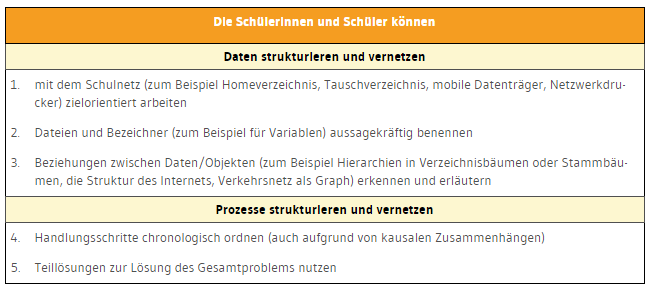
\includegraphics[width=\textwidth,height=\textheight,keepaspectratio]{images/struc.png}
	\caption{Infografik zu den Kompetenzen der Schüler im Fach Informatik im Bereich Strukturieren und Vernetzen}
	\label{Strukturieren und Vernetzen Infografik}
\end{figure}

\subsubsection{Modellieren und Implementieren}

Im Teilgebiet zu Modelieren und Implementieren lernen die Schüler die Kompetenzen um Problemstellungen aufzubereiten und daraus Modelle zu erstellen. Dabei stehen sowohl konstruierte Probleme als auch um Probleme aus der realen Welt im Fokus. Diese Modelle sollen auch implementiert und sinnvoll getestet werden um damit die Erstellung eines informatischen Systems abzuschließen. Der Bildungsplan sieht hierbei vor die spielerisch-probierende Ansätze zu verwenden und sowohl planvoll als auch strukturiert vorzugehen. Der Kerngedanke dieser Kompotenz soll es also sein, den Schülern beizubringen wie man von der Modelierung eines Problems Schrittweiße sich eine Lösung erarbeitet und diese Lösung danch überprüft. \cite{Model}.

\begin{figure}[H]
	\centering
	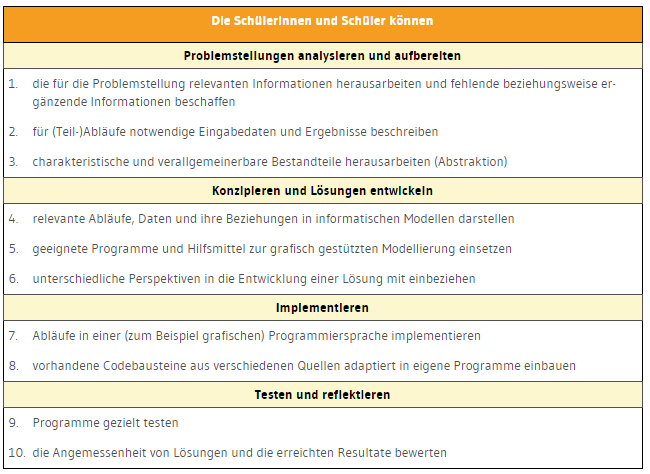
\includegraphics[width=\textwidth,height=\textheight,keepaspectratio]{images/model.png}
	\caption{Infografik zu den Kompetenzen der Schüler im Fach Informatik im Bereich Modellieren und Implementieren}
	\label{Modellieren und Implementieren Infografik}
\end{figure}

\subsubsection{Kommunizieren und Kooperieren}

Mit der Kompetenz Kommunizieren und Kooperieren  sollen die Schüler lernen wie man im Team effizent und fachgerecht arbeitet. Mit der Verwendung von fachgerechter Sparche sollen die Schüler über Sachverhalte diskutieren und die daraus entstehenden Ideen, Beobachtungen, Lösungeswege und Ergebnisse dokumentieren können. Ebenso sollen sie über die geeigneten Medienkompetenzen verfügen das ganze für andere zu visualisieren und kommunizieren. Die Schüler sollen sich kritische mit Fragen auseinandersetzen die mit gesellschaftskritischen Themen der Infromatik in Verbindung stehen. Dabei sollen die Schüler auch lernen die rechtlichen Aspekte einer solchen Kooperation zu verstehen und zu beachten. Um eine kooperatives und kollaberatives Arbeitsumfeld zu schaffen sollen die Schüler ebenfalls lernen in einem Diskurs über unterschiedliche Meinungen, Ansichten und Lösungen, respektvoll und offen mit seinen Kokurenten umgeht und diesen mit Akzeptanz und Toleranz begegnet.
\cite{Model}.

\begin{figure}[H]
	\centering
	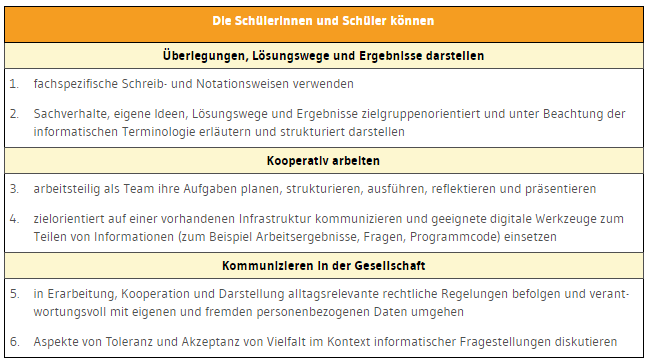
\includegraphics[width=\textwidth,height=\textheight,keepaspectratio]{images/team.png}
	\caption{Infografik zu den Kompetenzen der Schüler im Fach Informatik im Bereich Kommunizieren und Kooperieren}
	\label{Kommunizieren und Kooperieren Infografik}
\end{figure}

\subsubsection{Analysieren und Bewerten}

Das Analysieren und Bewerten von eigenen, sowie fremden System gehört ebenfalls zum Bildungsplan und ist in der Kompetenz Analysieren und Bewerten verankert. Die Schüler sollen hierbei lernen, wie man Programmcode analysiert, die Kontrollstrukturen identifieziert und Schrittwese nachvollzieht bis man die volle Funktionalität eines Programms versteht. Die schüler sind dabei ebenfalls in der Lage die sicherheitskritsche Probelme zu erkennen und diese gegebenfalls zu lösen und dabei gesellschaftliche, ethnische und technische Aspekte zu beachten.
\cite{Analy}.

\begin{figure}[H]
	\centering
	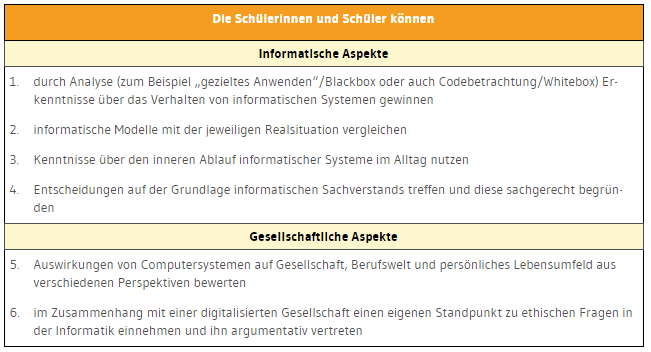
\includegraphics[width=\textwidth,height=\textheight,keepaspectratio]{images/Analysieren.png}
	\caption{Infografik zu den Kompetenzen der Schüler im Fach Informatik im Bereich Analysieren und Bewerten}
	\label{Analysieren und Bewerten Infografik}
\end{figure}

\subsubsection{Daten und Codierung}

Durch die Kompetenz Daten und Codierung sollen die Schüler ausgehend von alltäglichen Codierungen(wie z.B: KFZ-Kennzeichen oder Barcodes) eine zugrunde liegende Codierungsvorschrift herausarbeiten. Ebenso sollen sie in der Lage sein bestehende Codierungen wie z.B. Morsecode nach einer Einführung anwenden und verstehen zu können. Die Schüler lernen wie Computer und Maschinen verarbeiten und übertragen, Anhand von Erklärungen zu einfachen Codierungen wie dem Binärsystem oder der ASCII-Codierung. Dabei werden sich auf mit den gegnwärtigen Einheiten und Größenangaben der Datenhaltung( z.B: was bedeutetes wenn eine Datenträger eine Kapazität von "8 GB" besitzt?). \cite{Daten}.

\subsubsection{Algorithemn}

Durch diese Kompetenz soll den Schülern anhand von bekanten Arbeitsabläufen aus der realen Welt beigebracht werden was ein Algorithmus ist und wie man mit diesem durch formalisierte Handlungsweisen zur Lösung von einem Problem kommt. Die Schüler sollen selber lernen wie man mithilfe von elementarern Anweisungen und Kontrollstrukturen Alogrithmen beschreibt und wie man mit Variablen als änderbaren Wertespeicher einen Algorithmuss auch auf veränderte Probleme anwenden kann. Dabei werden die Schüler unterrichtet wie Alogrithmen mit geeigneten grafischen Veranschaulichungen(Struktogramme/Flussdiagramme) verständliche dargestellt werden können. Das ganze sollen die Schüler dann auch mit einer (vorzugsweise visuellen) Programmierumgebung implementieren und nachvollziehen können. Zu dieser Kompetenz zählt ebenfalls den Gesamtprozess von Problemanalyse bis hin zur Implementierung under Verifikation eines Problems zu kennen. Die Schüler sollen ein Bewusstsein über die zunehmende Bedeutung von Algorithmen im Alltag entwickeln.
\cite{Algo}.

\subsubsection{Rechner und Netze}

Mit der Kompetenz Rechner und Netze sollen die Schüler lernen wie die digitale Kommunikation funktioniert und die zugrunde liegenden Ideen davon kennenlernen. Sie erhalten einen groben überblick darüber wie die alltäglichen Kommunikationsvorgänge im Internet funktionieren und wie dessen Netze aufgebaut sind. Dabei lernen die Schüler wie ihre eigenen Endgeräte als Teil des ganzen Internets funktionieren und mit welchen Arten von Datenspeicherung und Datentransport diese arbeiten.
\cite{Rechner}.

\subsubsection{Informationsgesellschaft und Datensicherheit}

Mit dem Wissen aus der Kompetenz Rechner und Netze sollen die Schüler ein erweitertes Bewusstsein über Notwendigkeit erlangen, Daten gegen unbefugten Nutzen zu schützen. Sie sollen ein Verständiss dafür entwickeln, wie wichtig es in der Informationsgesellschaft ist die Anforderungen an die Verfügbarkeit , Vertraulichkeit und Integrität von Daten zu schützen und wie jeder einzelne die Verantowrtung über seine Daten trägt. Im Zuge dessen sollen die Schüler die Verschlüsselungsverfahren kennenlernen und wie man diese auch brechen kann, um so einen Einblick in das Teilgebiet der Kryptologie zu bekommen. Die Schüller sollen außerdem über die rechtlichen Hintergründe des Datenschutz aufgeklärt werden. Die Schüler sollen lernen konstruktiv und kritisch über die ethnischen und sozialen Aspekte des Datenschutzes diskutieren können und die verschiedenen Aspekte und Maßnahmen im Bezug auf den Datenschutz kennenlernen.
\cite{InfoGes}.

\subsection{Fazit}
Nach der Erläuterung des aktuellen Bildungsplans sind einige aus der Einleitung genannten Punkte doch breits schon umgesetzt worden. Aberes ist natürlich auch nicht davon ausgehen, dass ein Fach auch genau so unterrichtet wird, wie es im Bildungsplan vorgeschrieben wird. Theorie und Praxis unterscheiden sich in der Realität öfters und es gibt noch viele andere Faktoren die sich auf den Lerninhalt eines Schüler auswriken, wie z.B. Die Kompetenz des Lehrers oder der Wille zu Lernen bei den Schülern. Ein weiterere recht auffälliger Punkt, der bei der Aufkam war, dass der vorherige Bildungsplan zum Bildungsplan 2016 aus dem Jahr 2004 stammt. Wenn dieses Tempo beibehalten wird, kann man nicht vor dem Jahr 2028 mit einem neuen Bildungsplan rechnen. Im Feld der Informatik kann man es sich aber einfach nicht Leisten 12 Jahre lang nichts zu tun, während sich in der neue Technologien entwicklen und neue Paradigmen entstehen, während die alten langsam an relevanz verlieren und schließlich verschwinden. Deshalb sollte sich ein Bildungsplan in deutlich kleineren Abständen erneuern, wenn der Ziel doch sein soll, die nächste Generation auf die Real Welt loszulassen. Ein großer Punkt aus der Einleitung der nicht vom Bildungsplan abgedeckt wird ist eine Form von Logik-Unterricht und allgemein Fächer oder EInheiten in der Grundschule die mit Informatik oder Logik zu tun haben. Deshalb wäre genau das ein Potential das man noch erarbeiten könnte.

\section{Logik-Unterricht in der Grundschule}
dat können die kleinen scheißer auch!